\documentclass[]{article}
\usepackage{lmodern}
\usepackage{amssymb,amsmath}
\usepackage{ifxetex,ifluatex}
\usepackage{fixltx2e} % provides \textsubscript
\ifnum 0\ifxetex 1\fi\ifluatex 1\fi=0 % if pdftex
  \usepackage[T1]{fontenc}
  \usepackage[utf8]{inputenc}
\else % if luatex or xelatex
  \ifxetex
    \usepackage{mathspec}
  \else
    \usepackage{fontspec}
  \fi
  \defaultfontfeatures{Ligatures=TeX,Scale=MatchLowercase}
\fi
% use upquote if available, for straight quotes in verbatim environments
\IfFileExists{upquote.sty}{\usepackage{upquote}}{}
% use microtype if available
\IfFileExists{microtype.sty}{%
\usepackage{microtype}
\UseMicrotypeSet[protrusion]{basicmath} % disable protrusion for tt fonts
}{}
\usepackage[margin=1in]{geometry}
\usepackage{hyperref}
\hypersetup{unicode=true,
            pdftitle={Post Abril},
            pdfauthor={Dominic Royé},
            pdfborder={0 0 0},
            breaklinks=true}
\urlstyle{same}  % don't use monospace font for urls
\usepackage{color}
\usepackage{fancyvrb}
\newcommand{\VerbBar}{|}
\newcommand{\VERB}{\Verb[commandchars=\\\{\}]}
\DefineVerbatimEnvironment{Highlighting}{Verbatim}{commandchars=\\\{\}}
% Add ',fontsize=\small' for more characters per line
\usepackage{framed}
\definecolor{shadecolor}{RGB}{248,248,248}
\newenvironment{Shaded}{\begin{snugshade}}{\end{snugshade}}
\newcommand{\KeywordTok}[1]{\textcolor[rgb]{0.13,0.29,0.53}{\textbf{#1}}}
\newcommand{\DataTypeTok}[1]{\textcolor[rgb]{0.13,0.29,0.53}{#1}}
\newcommand{\DecValTok}[1]{\textcolor[rgb]{0.00,0.00,0.81}{#1}}
\newcommand{\BaseNTok}[1]{\textcolor[rgb]{0.00,0.00,0.81}{#1}}
\newcommand{\FloatTok}[1]{\textcolor[rgb]{0.00,0.00,0.81}{#1}}
\newcommand{\ConstantTok}[1]{\textcolor[rgb]{0.00,0.00,0.00}{#1}}
\newcommand{\CharTok}[1]{\textcolor[rgb]{0.31,0.60,0.02}{#1}}
\newcommand{\SpecialCharTok}[1]{\textcolor[rgb]{0.00,0.00,0.00}{#1}}
\newcommand{\StringTok}[1]{\textcolor[rgb]{0.31,0.60,0.02}{#1}}
\newcommand{\VerbatimStringTok}[1]{\textcolor[rgb]{0.31,0.60,0.02}{#1}}
\newcommand{\SpecialStringTok}[1]{\textcolor[rgb]{0.31,0.60,0.02}{#1}}
\newcommand{\ImportTok}[1]{#1}
\newcommand{\CommentTok}[1]{\textcolor[rgb]{0.56,0.35,0.01}{\textit{#1}}}
\newcommand{\DocumentationTok}[1]{\textcolor[rgb]{0.56,0.35,0.01}{\textbf{\textit{#1}}}}
\newcommand{\AnnotationTok}[1]{\textcolor[rgb]{0.56,0.35,0.01}{\textbf{\textit{#1}}}}
\newcommand{\CommentVarTok}[1]{\textcolor[rgb]{0.56,0.35,0.01}{\textbf{\textit{#1}}}}
\newcommand{\OtherTok}[1]{\textcolor[rgb]{0.56,0.35,0.01}{#1}}
\newcommand{\FunctionTok}[1]{\textcolor[rgb]{0.00,0.00,0.00}{#1}}
\newcommand{\VariableTok}[1]{\textcolor[rgb]{0.00,0.00,0.00}{#1}}
\newcommand{\ControlFlowTok}[1]{\textcolor[rgb]{0.13,0.29,0.53}{\textbf{#1}}}
\newcommand{\OperatorTok}[1]{\textcolor[rgb]{0.81,0.36,0.00}{\textbf{#1}}}
\newcommand{\BuiltInTok}[1]{#1}
\newcommand{\ExtensionTok}[1]{#1}
\newcommand{\PreprocessorTok}[1]{\textcolor[rgb]{0.56,0.35,0.01}{\textit{#1}}}
\newcommand{\AttributeTok}[1]{\textcolor[rgb]{0.77,0.63,0.00}{#1}}
\newcommand{\RegionMarkerTok}[1]{#1}
\newcommand{\InformationTok}[1]{\textcolor[rgb]{0.56,0.35,0.01}{\textbf{\textit{#1}}}}
\newcommand{\WarningTok}[1]{\textcolor[rgb]{0.56,0.35,0.01}{\textbf{\textit{#1}}}}
\newcommand{\AlertTok}[1]{\textcolor[rgb]{0.94,0.16,0.16}{#1}}
\newcommand{\ErrorTok}[1]{\textcolor[rgb]{0.64,0.00,0.00}{\textbf{#1}}}
\newcommand{\NormalTok}[1]{#1}
\usepackage{longtable,booktabs}
\usepackage{graphicx,grffile}
\makeatletter
\def\maxwidth{\ifdim\Gin@nat@width>\linewidth\linewidth\else\Gin@nat@width\fi}
\def\maxheight{\ifdim\Gin@nat@height>\textheight\textheight\else\Gin@nat@height\fi}
\makeatother
% Scale images if necessary, so that they will not overflow the page
% margins by default, and it is still possible to overwrite the defaults
% using explicit options in \includegraphics[width, height, ...]{}
\setkeys{Gin}{width=\maxwidth,height=\maxheight,keepaspectratio}
\IfFileExists{parskip.sty}{%
\usepackage{parskip}
}{% else
\setlength{\parindent}{0pt}
\setlength{\parskip}{6pt plus 2pt minus 1pt}
}
\setlength{\emergencystretch}{3em}  % prevent overfull lines
\providecommand{\tightlist}{%
  \setlength{\itemsep}{0pt}\setlength{\parskip}{0pt}}
\setcounter{secnumdepth}{0}
% Redefines (sub)paragraphs to behave more like sections
\ifx\paragraph\undefined\else
\let\oldparagraph\paragraph
\renewcommand{\paragraph}[1]{\oldparagraph{#1}\mbox{}}
\fi
\ifx\subparagraph\undefined\else
\let\oldsubparagraph\subparagraph
\renewcommand{\subparagraph}[1]{\oldsubparagraph{#1}\mbox{}}
\fi

%%% Use protect on footnotes to avoid problems with footnotes in titles
\let\rmarkdownfootnote\footnote%
\def\footnote{\protect\rmarkdownfootnote}

%%% Change title format to be more compact
\usepackage{titling}

% Create subtitle command for use in maketitle
\providecommand{\subtitle}[1]{
  \posttitle{
    \begin{center}\large#1\end{center}
    }
}

\setlength{\droptitle}{-2em}

  \title{Post Abril}
    \pretitle{\vspace{\droptitle}\centering\huge}
  \posttitle{\par}
    \author{Dominic Royé}
    \preauthor{\centering\large\emph}
  \postauthor{\par}
      \predate{\centering\large\emph}
  \postdate{\par}
    \date{18 de abril de 2019}


\begin{document}
\maketitle

Cuando pretendemos estimar la correlación entre múltiples variables, la
tarea se complica para obtener un resultado simple y limpio. Una forma
sencilla es usar la función \texttt{tidy()} del paquete
\emph{\{broom\}}. Como ejemplo, en este post vamos a estimar la
correlación entre la precipitación anual de varias ciudades españolas y
varios índices de teleconexiones climáticas:
\href{/files/teleconnections_indices.zip}{descarga}. Los datos de las
teleconexiones están preprocesados, pero pueden ser descargados
directamente desde
\href{https://crudata.uea.ac.uk/cru/data/pci.htm}{crudata.uea.ac.uk}. La
preciptiación proviene de
\href{https://www.ecad.eu//dailydata/index.php}{ECA\&D}.

\subsection{Paquetes}\label{paquetes}

En este post usaremos los siguientes paquetes:

\begin{longtable}[]{@{}ll@{}}
\toprule
Paquete & Descripción\tabularnewline
\midrule
\endhead
tidyverse & Conjunto de paquetes (visualización y manipulación de
datos): ggplot2, dplyr, purrr,etc.\tabularnewline
broom & Convierte resultados de funciones estadísticas (lm, t.test,
cor.test, etc.) en bonitas tablas\tabularnewline
fs & Proporciona una interfaz uniforme y multiplataforma para las
operaciones del sistema de archivos\tabularnewline
lubridate & Fácil manipulación de fechas y tiempos\tabularnewline
\bottomrule
\end{longtable}

\begin{Shaded}
\begin{Highlighting}[]
\CommentTok{#instalamos los paquetes si hace falta}
\ControlFlowTok{if}\NormalTok{(}\OperatorTok{!}\KeywordTok{require}\NormalTok{(}\StringTok{"tidyverse"}\NormalTok{)) }\KeywordTok{install.packages}\NormalTok{(}\StringTok{"tidyverse"}\NormalTok{)}
\ControlFlowTok{if}\NormalTok{(}\OperatorTok{!}\KeywordTok{require}\NormalTok{(}\StringTok{"broom"}\NormalTok{)) }\KeywordTok{install.packages}\NormalTok{(}\StringTok{"broom"}\NormalTok{)}
\ControlFlowTok{if}\NormalTok{(}\OperatorTok{!}\KeywordTok{require}\NormalTok{(}\StringTok{"fs"}\NormalTok{)) }\KeywordTok{install.packages}\NormalTok{(}\StringTok{"fs"}\NormalTok{)}
\ControlFlowTok{if}\NormalTok{(}\OperatorTok{!}\KeywordTok{require}\NormalTok{(}\StringTok{"lubridate"}\NormalTok{)) }\KeywordTok{install.packages}\NormalTok{(}\StringTok{"lubridate"}\NormalTok{)}

\CommentTok{#librerías}
\KeywordTok{library}\NormalTok{(tidyverse)}
\KeywordTok{library}\NormalTok{(broom)}
\KeywordTok{library}\NormalTok{(fs)}
\KeywordTok{library}\NormalTok{(lubridate)}
\end{Highlighting}
\end{Shaded}

\subsection{Importar datos}\label{importar-datos}

Primero debemos importar la precipitación diaria de las estaciones
meteorológicas seleccionadas.

\begin{enumerate}
\def\labelenumi{\arabic{enumi}.}
\item
  Creamos un vector con todos los archivos de precipitación con la
  función \texttt{dir\_ls()} del paquete \emph{\{fs\}}.
\item
  Importamos los datos con ayuda de la función \texttt{map\_df()} del
  paquete \emph{\{purrr\}} que aplica otra función a un vector o lista,
  y los une en una única tabla.
\item
  \begin{enumerate}
  \def\labelenumii{\alph{enumii})}
  \tightlist
  \item
    Seleccionamos únicamente las columnas que nos interesan, b)
    Convertimos la fecha en objeto \emph{date} con la función
    \texttt{ymd()} del paquete \emph{\{lubridate\}}, c) Creamos una
    nueva columna \emph{yr} con el año, d) Dividimos la precipitación
    entre 10 y reclasificamos valores ausentes -9999 por NA, e) Por
    último, reclasificamos la ID de cada estación meteorológica, creando
    un factor con nuevas etiquetas.
  \end{enumerate}
\end{enumerate}

Más detalles sobre el uso de las funciones \texttt{dir\_ls()} y
\texttt{map\_df()} en este último
\href{https://dominicroye.github.io/en/2019/import-excel-sheets-with-r/}{post}.

\begin{Shaded}
\begin{Highlighting}[]
\CommentTok{#archivos de la precipitación}
\NormalTok{files <-}\StringTok{ }\KeywordTok{dir_ls}\NormalTok{(}\DataTypeTok{regexp =} \StringTok{"txt"}\NormalTok{)}
\NormalTok{files}
\end{Highlighting}
\end{Shaded}

\begin{verbatim}
## RR_STAID001393.txt RR_STAID001394.txt RR_STAID002969.txt 
## RR_STAID003946.txt RR_STAID003969.txt
\end{verbatim}

\begin{Shaded}
\begin{Highlighting}[]
\CommentTok{#importamos todos, uniéndolos en una única tabla}
\NormalTok{pr <-}\StringTok{ }\NormalTok{files }\OperatorTok\StringTok{ }\KeywordTok{map_df}\NormalTok{(read_csv,}\DataTypeTok{skip=}\DecValTok{20}\NormalTok{)}
\end{Highlighting}
\end{Shaded}

\begin{verbatim}
## Parsed with column specification:
## cols(
##   STAID = col_double(),
##   SOUID = col_double(),
##   DATE = col_double(),
##   RR = col_double(),
##   Q_RR = col_double()
## )
## Parsed with column specification:
## cols(
##   STAID = col_double(),
##   SOUID = col_double(),
##   DATE = col_double(),
##   RR = col_double(),
##   Q_RR = col_double()
## )
## Parsed with column specification:
## cols(
##   STAID = col_double(),
##   SOUID = col_double(),
##   DATE = col_double(),
##   RR = col_double(),
##   Q_RR = col_double()
## )
## Parsed with column specification:
## cols(
##   STAID = col_double(),
##   SOUID = col_double(),
##   DATE = col_double(),
##   RR = col_double(),
##   Q_RR = col_double()
## )
## Parsed with column specification:
## cols(
##   STAID = col_double(),
##   SOUID = col_double(),
##   DATE = col_double(),
##   RR = col_double(),
##   Q_RR = col_double()
## )
\end{verbatim}

\begin{Shaded}
\begin{Highlighting}[]
\NormalTok{pr}
\end{Highlighting}
\end{Shaded}

\begin{verbatim}
## # A tibble: 133,343 x 5
##    STAID SOUID     DATE    RR  Q_RR
##    <dbl> <dbl>    <dbl> <dbl> <dbl>
##  1  1393 20611 19470301     0     0
##  2  1393 20611 19470302     5     0
##  3  1393 20611 19470303     0     0
##  4  1393 20611 19470304    33     0
##  5  1393 20611 19470305    15     0
##  6  1393 20611 19470306     0     0
##  7  1393 20611 19470307    85     0
##  8  1393 20611 19470308     3     0
##  9  1393 20611 19470309     0     0
## 10  1393 20611 19470310     0     0
## # ... with 133,333 more rows
\end{verbatim}

\begin{Shaded}
\begin{Highlighting}[]
\CommentTok{#creamos los niveles del factor }
\NormalTok{id <-}\StringTok{ }\KeywordTok{unique}\NormalTok{(pr}\OperatorTok{$}\NormalTok{STAID)}

\CommentTok{#las etiquetas correspondientes}
\NormalTok{lab <-}\StringTok{ }\KeywordTok{c}\NormalTok{(}\StringTok{"Bilbao"}\NormalTok{,}\StringTok{"Santiago"}\NormalTok{,}\StringTok{"Barcelona"}\NormalTok{,}\StringTok{"Madrid"}\NormalTok{,}\StringTok{"Valencia"}\NormalTok{)}

\CommentTok{#primeros cambios}
\NormalTok{pr <-}\StringTok{ }\KeywordTok{select}\NormalTok{(pr,STAID,DATE,RR)}\OperatorTok\StringTok{ }
\StringTok{        }\KeywordTok{mutate}\NormalTok{(}\DataTypeTok{DATE=}\KeywordTok{ymd}\NormalTok{(DATE), }
               \DataTypeTok{RR=}\KeywordTok{ifelse}\NormalTok{(RR}\OperatorTok{==-}\DecValTok{9999}\NormalTok{,}\OtherTok{NA}\NormalTok{,RR}\OperatorTok{/}\DecValTok{10}\NormalTok{), }
               \DataTypeTok{STAID=}\KeywordTok{factor}\NormalTok{(STAID,id,lab), }
               \DataTypeTok{yr=}\KeywordTok{year}\NormalTok{(DATE)) }
\NormalTok{pr}
\end{Highlighting}
\end{Shaded}

\begin{verbatim}
## # A tibble: 133,343 x 4
##    STAID  DATE          RR    yr
##    <fct>  <date>     <dbl> <dbl>
##  1 Bilbao 1947-03-01   0    1947
##  2 Bilbao 1947-03-02   0.5  1947
##  3 Bilbao 1947-03-03   0    1947
##  4 Bilbao 1947-03-04   3.3  1947
##  5 Bilbao 1947-03-05   1.5  1947
##  6 Bilbao 1947-03-06   0    1947
##  7 Bilbao 1947-03-07   8.5  1947
##  8 Bilbao 1947-03-08   0.3  1947
##  9 Bilbao 1947-03-09   0    1947
## 10 Bilbao 1947-03-10   0    1947
## # ... with 133,333 more rows
\end{verbatim}

Lo que todavía nos hace falta es filtrar y calcular la suma anual de
precipitación. En principio, no es lo más correcto sumar la
precipitación sin tener en cuenta que haya valores ausentes, pero nos
sirve igualmente para este ensayo. Después, cambiamos el formato de la
tabla con la función \texttt{spread()}, pasando de una tabla larga a una
ancha, es decir, queremos obtener una columna por estación
meteorológica.

\begin{Shaded}
\begin{Highlighting}[]
\NormalTok{pr_yr <-}\StringTok{ }\KeywordTok{filter}\NormalTok{(pr,DATE}\OperatorTok{>=}\StringTok{"1950-01-01"}\NormalTok{,DATE}\OperatorTok{<}\StringTok{"2018-01-01"}\NormalTok{)}\OperatorTok
\StringTok{           }\KeywordTok{group_by}\NormalTok{(STAID,yr)}\OperatorTok
\StringTok{             }\KeywordTok{summarise}\NormalTok{(}\DataTypeTok{pr=}\KeywordTok{sum}\NormalTok{(RR,}\DataTypeTok{na.rm =} \OtherTok{TRUE}\NormalTok{))}
\NormalTok{pr_yr}
\end{Highlighting}
\end{Shaded}

\begin{verbatim}
## # A tibble: 324 x 3
## # Groups:   STAID [5]
##    STAID     yr    pr
##    <fct>  <dbl> <dbl>
##  1 Bilbao  1950 1342 
##  2 Bilbao  1951 1306.
##  3 Bilbao  1952 1355.
##  4 Bilbao  1953 1372.
##  5 Bilbao  1954 1428.
##  6 Bilbao  1955 1062.
##  7 Bilbao  1956 1254.
##  8 Bilbao  1957  968.
##  9 Bilbao  1958 1272.
## 10 Bilbao  1959 1450.
## # ... with 314 more rows
\end{verbatim}

\begin{Shaded}
\begin{Highlighting}[]
\NormalTok{pr_yr <-}\StringTok{ }\KeywordTok{spread}\NormalTok{(pr_yr,STAID,pr)}
\NormalTok{pr_yr}
\end{Highlighting}
\end{Shaded}

\begin{verbatim}
## # A tibble: 68 x 6
##       yr Bilbao Santiago Barcelona Madrid Valencia
##    <dbl>  <dbl>    <dbl>     <dbl>  <dbl>    <dbl>
##  1  1950  1342     1800.      345     NA        NA
##  2  1951  1306.    2344.     1072.   798.       NA
##  3  1952  1355.    1973.      415.   524.       NA
##  4  1953  1372.     973.      683.   365.       NA
##  5  1954  1428.    1348.      581.   246.       NA
##  6  1955  1062.    1769.      530.   473.       NA
##  7  1956  1254.    1533.      695.   480.       NA
##  8  1957   968.    1599.      635.   424.       NA
##  9  1958  1272.    2658.      479.   482.       NA
## 10  1959  1450.    2847.     1006    665.       NA
## # ... with 58 more rows
\end{verbatim}

El siguiente paso es importar los índices de las teleconexiones.

\begin{Shaded}
\begin{Highlighting}[]
\CommentTok{#teleconexiones}
\NormalTok{telecon <-}\StringTok{ }\KeywordTok{read_csv}\NormalTok{(}\StringTok{"teleconnections_indices.csv"}\NormalTok{)}
\end{Highlighting}
\end{Shaded}

\begin{verbatim}
## Parsed with column specification:
## cols(
##   yr = col_double(),
##   NAO = col_double(),
##   WeMO = col_double(),
##   EA = col_double(),
##   `POL-EUAS` = col_double(),
##   `EATL/WRUS` = col_double(),
##   MO = col_double(),
##   SCAND = col_double(),
##   AO = col_double()
## )
\end{verbatim}

\begin{Shaded}
\begin{Highlighting}[]
\NormalTok{telecon}
\end{Highlighting}
\end{Shaded}

\begin{verbatim}
## # A tibble: 68 x 9
##       yr   NAO   WeMO     EA `POL-EUAS` `EATL/WRUS`    MO    SCAND       AO
##    <dbl> <dbl>  <dbl>  <dbl>      <dbl>       <dbl> <dbl>    <dbl>    <dbl>
##  1  1950  0.49  0.555 -0.332     0.0217     -0.0567 0.335  0.301   -1.99e-1
##  2  1951 -0.07  0.379 -0.372     0.402      -0.419  0.149 -0.00667 -3.65e-1
##  3  1952 -0.37  0.693 -0.688    -0.0117     -0.711  0.282  0.0642  -6.75e-1
##  4  1953  0.4  -0.213 -0.727    -0.0567     -0.0508 0.216  0.0233  -1.64e-2
##  5  1954  0.51  1.20  -0.912     0.142      -0.318  0.386  0.458   -5.83e-4
##  6  1955 -0.64  0.138 -0.824    -0.0267      0.154  0.134  0.0392  -3.62e-1
##  7  1956  0.17  0.617 -1.29     -0.197       0.0617 0.256  0.302   -1.63e-1
##  8  1957 -0.02  0.321 -0.952    -0.638      -0.167  0.322 -0.134   -3.42e-1
##  9  1958  0.12  0.941 -0.243     0.138       0.661  0.296  0.279   -8.68e-1
## 10  1959  0.49 -0.055 -0.23     -0.0142      0.631  0.316  0.725   -7.62e-2
## # ... with 58 more rows
\end{verbatim}

Por último nos falta unir ambas tablas por año.

\begin{Shaded}
\begin{Highlighting}[]
\NormalTok{data_all <-}\StringTok{ }\KeywordTok{left_join}\NormalTok{(pr_yr,telecon,}\DataTypeTok{by=}\StringTok{"yr"}\NormalTok{)}
\NormalTok{data_all}
\end{Highlighting}
\end{Shaded}

\begin{verbatim}
## # A tibble: 68 x 14
##       yr Bilbao Santiago Barcelona Madrid Valencia   NAO   WeMO     EA
##    <dbl>  <dbl>    <dbl>     <dbl>  <dbl>    <dbl> <dbl>  <dbl>  <dbl>
##  1  1950  1342     1800.      345     NA        NA  0.49  0.555 -0.332
##  2  1951  1306.    2344.     1072.   798.       NA -0.07  0.379 -0.372
##  3  1952  1355.    1973.      415.   524.       NA -0.37  0.693 -0.688
##  4  1953  1372.     973.      683.   365.       NA  0.4  -0.213 -0.727
##  5  1954  1428.    1348.      581.   246.       NA  0.51  1.20  -0.912
##  6  1955  1062.    1769.      530.   473.       NA -0.64  0.138 -0.824
##  7  1956  1254.    1533.      695.   480.       NA  0.17  0.617 -1.29 
##  8  1957   968.    1599.      635.   424.       NA -0.02  0.321 -0.952
##  9  1958  1272.    2658.      479.   482.       NA  0.12  0.941 -0.243
## 10  1959  1450.    2847.     1006    665.       NA  0.49 -0.055 -0.23 
## # ... with 58 more rows, and 5 more variables: `POL-EUAS` <dbl>,
## #   `EATL/WRUS` <dbl>, MO <dbl>, SCAND <dbl>, AO <dbl>
\end{verbatim}

\subsection{Test de correlación}\label{test-de-correlacion}

Un test de correlación lo podemos hacer con la función
\texttt{cor.test()} de \emph{R Base}. En este caso entre la
precipitación anual de Bilbao y el índice de NAO.

\begin{Shaded}
\begin{Highlighting}[]
\NormalTok{cor_nao_bil <-}\StringTok{ }\KeywordTok{cor.test}\NormalTok{(data_all}\OperatorTok{$}\NormalTok{Bilbao,data_all}\OperatorTok{$}\NormalTok{NAO,}
                        \DataTypeTok{method=}\StringTok{"spearman"}\NormalTok{)}
\end{Highlighting}
\end{Shaded}

\begin{verbatim}
## Warning in cor.test.default(data_all$Bilbao, data_all$NAO, method =
## "spearman"): Cannot compute exact p-value with ties
\end{verbatim}

\begin{Shaded}
\begin{Highlighting}[]
\NormalTok{cor_nao_bil}
\end{Highlighting}
\end{Shaded}

\begin{verbatim}
## 
##  Spearman's rank correlation rho
## 
## data:  data_all$Bilbao and data_all$NAO
## S = 44372, p-value = 0.2126
## alternative hypothesis: true rho is not equal to 0
## sample estimates:
##       rho 
## 0.1531149
\end{verbatim}

Vemos que el resultado está en un formato poco manejable. Nos resume la
correlación con todos los parametros estadísticos necesarios para sacar
una conclusión sobre la relación. La función \texttt{tidy()} del paquete
\emph{\{broom\}} nos permite convertir el resultado en formato de tabla.

\begin{Shaded}
\begin{Highlighting}[]
\KeywordTok{tidy}\NormalTok{(cor_nao_bil)}
\end{Highlighting}
\end{Shaded}

\begin{verbatim}
## # A tibble: 1 x 5
##   estimate statistic p.value method                          alternative
##      <dbl>     <dbl>   <dbl> <chr>                           <chr>      
## 1    0.153    44372.   0.213 Spearman's rank correlation rho two.sided
\end{verbatim}

\subsection{Aplicar el test de correlación a múltiples
variables}\label{aplicar-el-test-de-correlacion-a-multiples-variables}

El objetivo es aplicar el test de correlación a todas las estaciones
meteorológicas e índices de teleconexiones.

Primero, debemos pasar la tabla al formato largo, o sea, crear una
columna de la ciudad y el valor de la precipitación correspondiente.
Después lo repetimos para las teleconexiones.

\begin{Shaded}
\begin{Highlighting}[]
\NormalTok{data <-}\StringTok{ }\KeywordTok{gather}\NormalTok{(data_all,city,pr,Bilbao}\OperatorTok{:}\NormalTok{Valencia)}\OperatorTok
\StringTok{                     }\KeywordTok{gather}\NormalTok{(telecon,index,NAO}\OperatorTok{:}\NormalTok{AO)}
\NormalTok{data}
\end{Highlighting}
\end{Shaded}

\begin{verbatim}
## # A tibble: 2,720 x 5
##       yr city      pr telecon index
##    <dbl> <chr>  <dbl> <chr>   <dbl>
##  1  1950 Bilbao 1342  NAO      0.49
##  2  1951 Bilbao 1306. NAO     -0.07
##  3  1952 Bilbao 1355. NAO     -0.37
##  4  1953 Bilbao 1372. NAO      0.4 
##  5  1954 Bilbao 1428. NAO      0.51
##  6  1955 Bilbao 1062. NAO     -0.64
##  7  1956 Bilbao 1254. NAO      0.17
##  8  1957 Bilbao  968. NAO     -0.02
##  9  1958 Bilbao 1272. NAO      0.12
## 10  1959 Bilbao 1450. NAO      0.49
## # ... with 2,710 more rows
\end{verbatim}

Para poder aplicar el test a todas las ciudades, debemos tener las
correspondientes agrupaciones. Por ello, usamos la función
\texttt{group\_by()} indicando los dos grupos (\emph{city} y
\emph{telecon}), y además, aplicamos la función \texttt{nest()} del
paquete \emph{\{tidyr\}}, colección \emph{\{tidyverse\}}, con el
objetivo de crear listas de tablas encajadas por fila. En otras
palabras, en cada fila de cada ciudad y teleconexión tendremos una nueva
tabla que contiene correspondientemente el año, la precipitación y el
valor del índice.

\begin{Shaded}
\begin{Highlighting}[]
\NormalTok{data_nest <-}\StringTok{ }\KeywordTok{group_by}\NormalTok{(data,city,telecon)}\OperatorTok\KeywordTok{nest}\NormalTok{()}
\NormalTok{data_nest}
\end{Highlighting}
\end{Shaded}

\begin{verbatim}
## # A tibble: 40 x 3
##    city      telecon data             
##    <chr>     <chr>   <list>           
##  1 Bilbao    NAO     <tibble [68 x 3]>
##  2 Santiago  NAO     <tibble [68 x 3]>
##  3 Barcelona NAO     <tibble [68 x 3]>
##  4 Madrid    NAO     <tibble [68 x 3]>
##  5 Valencia  NAO     <tibble [68 x 3]>
##  6 Bilbao    WeMO    <tibble [68 x 3]>
##  7 Santiago  WeMO    <tibble [68 x 3]>
##  8 Barcelona WeMO    <tibble [68 x 3]>
##  9 Madrid    WeMO    <tibble [68 x 3]>
## 10 Valencia  WeMO    <tibble [68 x 3]>
## # ... with 30 more rows
\end{verbatim}

\begin{Shaded}
\begin{Highlighting}[]
\KeywordTok{str}\NormalTok{(}\KeywordTok{slice}\NormalTok{(data_nest,}\DecValTok{1}\NormalTok{))}
\end{Highlighting}
\end{Shaded}

\begin{verbatim}
## Classes 'tbl_df', 'tbl' and 'data.frame':    1 obs. of  3 variables:
##  $ city   : chr "Bilbao"
##  $ telecon: chr "NAO"
##  $ data   :List of 1
##   ..$ :Classes 'tbl_df', 'tbl' and 'data.frame': 68 obs. of  3 variables:
##   .. ..$ yr   : num  1950 1951 1952 1953 1954 ...
##   .. ..$ pr   : num  1342 1306 1355 1372 1428 ...
##   .. ..$ index: num  0.49 -0.07 -0.37 0.4 0.51 -0.64 0.17 -0.02 0.12 0.49 ...
\end{verbatim}

El siguiente paso es crear una función, en la que definimos el test de
correlación y lo pasamos al formato limpio, que aplicamos a cada
agrupación.

\begin{Shaded}
\begin{Highlighting}[]
\NormalTok{cor_fun <-}\StringTok{ }\ControlFlowTok{function}\NormalTok{(df) }\KeywordTok{cor.test}\NormalTok{(df}\OperatorTok{$}\NormalTok{pr,df}\OperatorTok{$}\NormalTok{index,}\DataTypeTok{method=}\StringTok{"spearman"}\NormalTok{)}\OperatorTok\KeywordTok{tidy}\NormalTok{()}
\end{Highlighting}
\end{Shaded}

Ahora sólo nos queda por aplicar nuestra función a la columna que
contiene las tablas por cada combinación entre ciudad y teleconexión.
Para ello, usamos la función \texttt{map()} que aplica otra función
sobre un vector o lista. Lo que hacemos es crear una nueva columna que
contiene el resultado, una tabla del resumen estadístico, por cada fila
de cada combinación.

\begin{Shaded}
\begin{Highlighting}[]
\NormalTok{data_nest <-}\StringTok{ }\KeywordTok{mutate}\NormalTok{(data_nest, }\DataTypeTok{model =} \KeywordTok{map}\NormalTok{(data,cor_fun))}
\NormalTok{data_nest}
\end{Highlighting}
\end{Shaded}

\begin{verbatim}
## # A tibble: 40 x 4
##    city      telecon data              model           
##    <chr>     <chr>   <list>            <list>          
##  1 Bilbao    NAO     <tibble [68 x 3]> <tibble [1 x 5]>
##  2 Santiago  NAO     <tibble [68 x 3]> <tibble [1 x 5]>
##  3 Barcelona NAO     <tibble [68 x 3]> <tibble [1 x 5]>
##  4 Madrid    NAO     <tibble [68 x 3]> <tibble [1 x 5]>
##  5 Valencia  NAO     <tibble [68 x 3]> <tibble [1 x 5]>
##  6 Bilbao    WeMO    <tibble [68 x 3]> <tibble [1 x 5]>
##  7 Santiago  WeMO    <tibble [68 x 3]> <tibble [1 x 5]>
##  8 Barcelona WeMO    <tibble [68 x 3]> <tibble [1 x 5]>
##  9 Madrid    WeMO    <tibble [68 x 3]> <tibble [1 x 5]>
## 10 Valencia  WeMO    <tibble [68 x 3]> <tibble [1 x 5]>
## # ... with 30 more rows
\end{verbatim}

\begin{Shaded}
\begin{Highlighting}[]
\KeywordTok{str}\NormalTok{(}\KeywordTok{slice}\NormalTok{(data_nest,}\DecValTok{1}\NormalTok{))}
\end{Highlighting}
\end{Shaded}

\begin{verbatim}
## Classes 'tbl_df', 'tbl' and 'data.frame':    1 obs. of  4 variables:
##  $ city   : chr "Bilbao"
##  $ telecon: chr "NAO"
##  $ data   :List of 1
##   ..$ :Classes 'tbl_df', 'tbl' and 'data.frame': 68 obs. of  3 variables:
##   .. ..$ yr   : num  1950 1951 1952 1953 1954 ...
##   .. ..$ pr   : num  1342 1306 1355 1372 1428 ...
##   .. ..$ index: num  0.49 -0.07 -0.37 0.4 0.51 -0.64 0.17 -0.02 0.12 0.49 ...
##  $ model  :List of 1
##   ..$ :Classes 'tbl_df', 'tbl' and 'data.frame': 1 obs. of  5 variables:
##   .. ..$ estimate   : num 0.153
##   .. ..$ statistic  : num 44372
##   .. ..$ p.value    : num 0.213
##   .. ..$ method     : chr "Spearman's rank correlation rho"
##   .. ..$ alternative: chr "two.sided"
\end{verbatim}

¿Cómo podemos deshacer la lista de tablas en cada fila de nuestra tabla?

Pues bien, primero eliminamos la columna con los datos y después
aplicamos simplemente la función \texttt{unnest()}.

\begin{Shaded}
\begin{Highlighting}[]
\NormalTok{corr_pr <-}\StringTok{ }\KeywordTok{select}\NormalTok{(data_nest,}\OperatorTok{-}\NormalTok{data)}\OperatorTok\KeywordTok{unnest}\NormalTok{()}
\NormalTok{corr_pr}
\end{Highlighting}
\end{Shaded}

\begin{verbatim}
## # A tibble: 40 x 7
##    city    telecon estimate statistic  p.value method           alternative
##    <chr>   <chr>      <dbl>     <dbl>    <dbl> <chr>            <chr>      
##  1 Bilbao  NAO       0.153     44372. 0.213    Spearman's rank~ two.sided  
##  2 Santia~ NAO      -0.181     61902. 0.139    Spearman's rank~ two.sided  
##  3 Barcel~ NAO      -0.0203    53460. 0.869    Spearman's rank~ two.sided  
##  4 Madrid  NAO      -0.291     64692. 0.0169   Spearman's rank~ two.sided  
##  5 Valenc~ NAO      -0.113     27600. 0.422    Spearman's rank~ two.sided  
##  6 Bilbao  WeMO      0.404     31242. 0.000706 Spearman's rank~ two.sided  
##  7 Santia~ WeMO      0.332     35014. 0.00594  Spearman's rank~ two.sided  
##  8 Barcel~ WeMO      0.0292    50862  0.813    Spearman's rank~ two.sided  
##  9 Madrid  WeMO      0.109     44660  0.380    Spearman's rank~ two.sided  
## 10 Valenc~ WeMO     -0.252     31056. 0.0688   Spearman's rank~ two.sided  
## # ... with 30 more rows
\end{verbatim}

El resultado es una tabla en la que podemos ver las correlaciones y su
significación estadística para cada ciudad y teleconexiones.

\subsection{Heatmap de los resultados}\label{heatmap-de-los-resultados}

Finalmente, hacemos un \emph{heatmap} del resultado obtenido. Antes
creamos una columna que indica si la correlación es significativa con
p-valor menor de 0,05.

\begin{Shaded}
\begin{Highlighting}[]
\NormalTok{corr_pr <-}\StringTok{ }\KeywordTok{mutate}\NormalTok{(corr_pr,}\DataTypeTok{sig=}\KeywordTok{ifelse}\NormalTok{(p.value}\OperatorTok{<}\FloatTok{0.05}\NormalTok{,}\StringTok{"Sig."}\NormalTok{,}\StringTok{"Non Sig."}\NormalTok{))}
\end{Highlighting}
\end{Shaded}

\begin{Shaded}
\begin{Highlighting}[]
\KeywordTok{ggplot}\NormalTok{()}\OperatorTok{+}
\StringTok{  }\KeywordTok{geom_tile}\NormalTok{(}\DataTypeTok{data=}\NormalTok{corr_pr,}
            \KeywordTok{aes}\NormalTok{(city,telecon,}\DataTypeTok{fill=}\NormalTok{estimate),}
            \DataTypeTok{size=}\DecValTok{1}\NormalTok{,}
            \DataTypeTok{colour=}\StringTok{"white"}\NormalTok{)}\OperatorTok{+}
\StringTok{  }\KeywordTok{geom_tile}\NormalTok{(}\DataTypeTok{data=}\KeywordTok{filter}\NormalTok{(corr_pr,sig}\OperatorTok{==}\StringTok{"Sig."}\NormalTok{),}
            \KeywordTok{aes}\NormalTok{(city,telecon),}
            \DataTypeTok{size=}\DecValTok{1}\NormalTok{,}
            \DataTypeTok{colour=}\StringTok{"black"}\NormalTok{,}
            \DataTypeTok{fill=}\StringTok{"transparent"}\NormalTok{)}\OperatorTok{+}
\StringTok{  }\KeywordTok{geom_text}\NormalTok{(}\DataTypeTok{data=}\NormalTok{corr_pr,}
            \KeywordTok{aes}\NormalTok{(city,telecon,}\DataTypeTok{label=}\KeywordTok{round}\NormalTok{(estimate,}\DecValTok{2}\NormalTok{),}
            \DataTypeTok{fontface=}\KeywordTok{ifelse}\NormalTok{(sig}\OperatorTok{==}\StringTok{"Sig."}\NormalTok{,}\StringTok{"bold"}\NormalTok{,}\StringTok{"plain"}\NormalTok{)))}\OperatorTok{+}
\StringTok{  }\KeywordTok{scale_fill_gradient2}\NormalTok{(}\DataTypeTok{breaks=}\KeywordTok{seq}\NormalTok{(}\OperatorTok{-}\DecValTok{1}\NormalTok{,}\DecValTok{1}\NormalTok{,}\FloatTok{0.2}\NormalTok{))}\OperatorTok{+}
\StringTok{  }\KeywordTok{labs}\NormalTok{(}\DataTypeTok{x=}\StringTok{""}\NormalTok{,}\DataTypeTok{y=}\StringTok{""}\NormalTok{,}\DataTypeTok{fill=}\StringTok{""}\NormalTok{,}\DataTypeTok{p.value=}\StringTok{""}\NormalTok{)}\OperatorTok{+}
\StringTok{  }\KeywordTok{theme_minimal}\NormalTok{()}\OperatorTok{+}
\StringTok{  }\KeywordTok{theme}\NormalTok{(}\DataTypeTok{panel.grid.major =} \KeywordTok{element_blank}\NormalTok{(),}
        \DataTypeTok{panel.border =} \KeywordTok{element_blank}\NormalTok{(),}
        \DataTypeTok{panel.background =} \KeywordTok{element_blank}\NormalTok{(),}
        \DataTypeTok{axis.ticks =} \KeywordTok{element_blank}\NormalTok{())}
\end{Highlighting}
\end{Shaded}

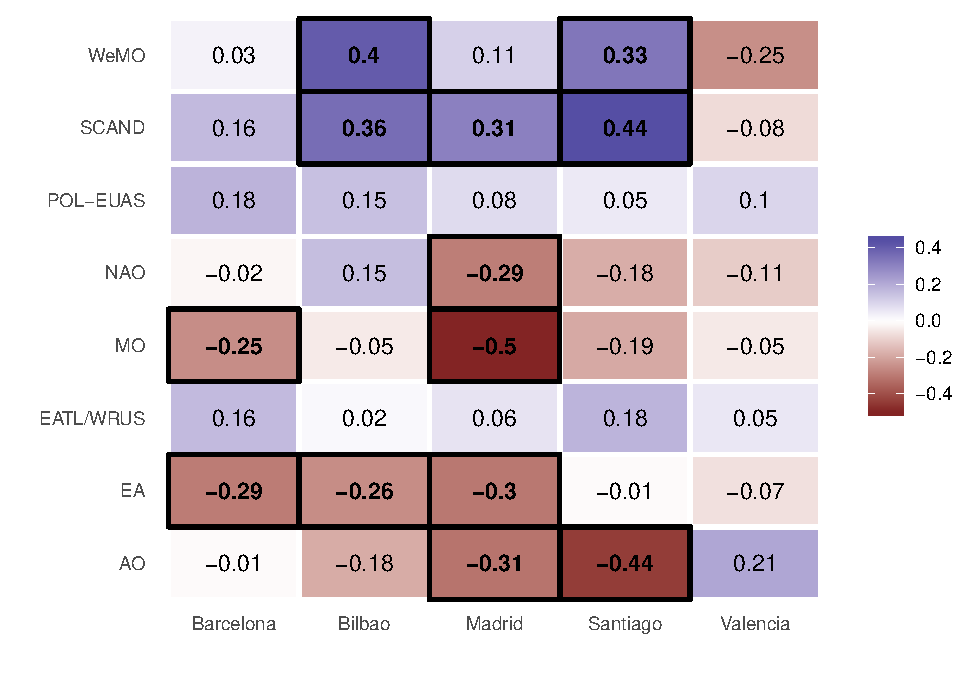
\includegraphics{post_abril_files/figure-latex/unnamed-chunk-15-1.pdf}


\end{document}
